\documentclass[border=0pt, tikz]{standalone}
\usepackage{color}
\usepackage{tikz}

\begin{document}
    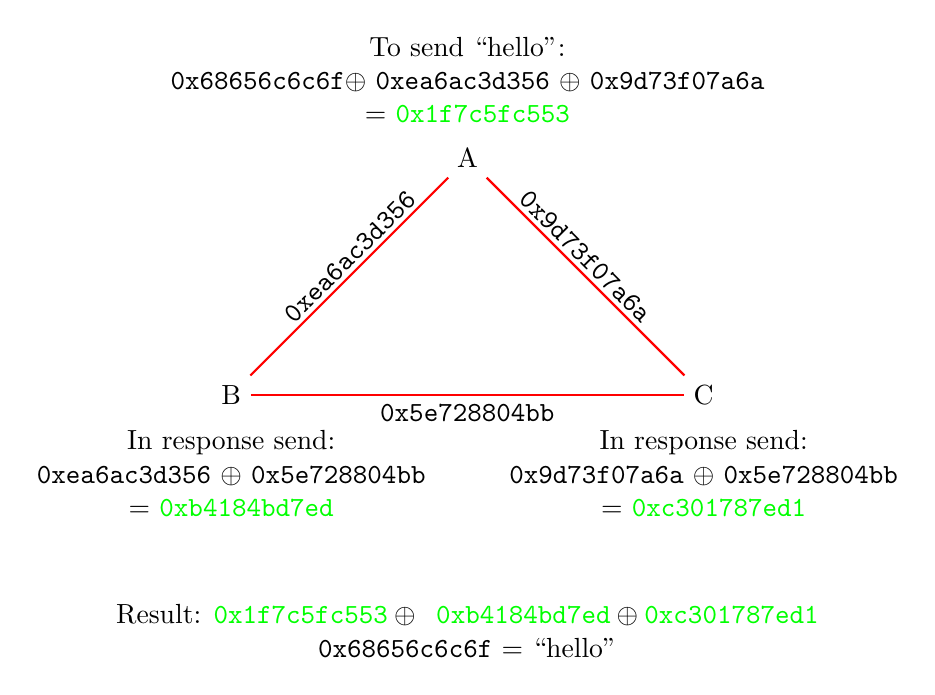
\begin{tikzpicture}[node distance = 3cm]
        \node (A) {A};
        \node [left of = A, below of = A] (B) {B};
        \node [right of = A, below of = A] (C) {C};

        \draw [thick, red] (A)--(B) node [sloped, black, pos=0.1, left,
        yshift=5pt] {\texttt{0xea6ac3d356}};
        \draw [thick, red] (B)--(C) node [sloped, black, pos=0.5, below] {
        \texttt{0x5e728804bb}};
        \draw [thick, red] (C)--(A) node [sloped, black, pos=0.9, above, right,
        yshift=5pt]{\texttt{0x9d73f07a6a}};
       

        \node [align=center,above of = A, node distance = 1cm] (_) 
        {To send ``hello'':\\\texttt{0x68656c6c6f}$\oplus$
        \texttt{0xea6ac3d356} $\oplus$ \texttt{0x9d73f07a6a}\\$=$
        \texttt{\color{green}0x1f7c5fc553}};

        \node [align=center, below of = B, node distance = 1cm] (_) 
        {In response send:\\\texttt{0xea6ac3d356} $\oplus$ 
        \texttt{0x5e728804bb}\\$=$ \texttt{\color{green}0xb4184bd7ed}};

        \node [align=center, below of = C, node distance = 1cm] (_) 
        {In response send:\\\texttt{0x9d73f07a6a} $\oplus$ 
        \texttt{0x5e728804bb}\\$=$ \texttt{\color{green}0xc301787ed1}};

        \node [align=center, below of = C, left of = C] (_) {Result: 
        $\texttt{\color{green}0x1f7c5fc553}\oplus \texttt{
        \color{green}0xb4184bd7ed} \oplus \texttt{\color{green}0xc301787ed1}
        $\\\color{black}\texttt{0x68656c6c6f} = ``hello''};
    \end{tikzpicture}
\end{document}
